\documentclass[a4paper,10pt]{article}
\usepackage[utf8x]{inputenc}
\usepackage{graphicx}
\usepackage{pgf}
\pgfdeclareimage[height=1cm]{myimage}{p1_q1.png}


%opening   
\title{ \textbf{Universidade de Brasília -- Faculdade do Gama \\ Sistemas digitais 2 \\ Lista 1 }}
\date{Setembro - 2011}

\begin{document}
\maketitle

\section{Parte 1}
\begin{enumerate}
 \item Construa uma máquina de estado finito que calcule x+1 onde x é dado na forma binária, com o bit-menos significativo primeiro.
 \item Você tem uma conta no Banco Nacional do Lucro Certo (BNLC) e um cartão para operar sua conta bancária. Uma vez introduzido seu cartão, a máquina do banco 
       permite processar uma transação apenas se você entrar seu código correto, que 417. Desenhe um diagrama de estados para uma máquina de estado finito desenhada 
       para reconhecer este código. O alfabeto de saída deve ter três símbolos de saída: “bingo” (código correto), “aguarde” (correto também) e “invalido” (código 
       incorreto). O alfabeto de entrada é {0, 1, 2, …, 9}. Para simplificar a notação, podemos nos referir a uma aresta por I-{3}, por exemplo, que significa que a 
       máquina percorrerá esta aresta para qualquer símbolo de entrada que não seja o 3. (No BNLC, você tem apenas uma chance de entrar seu código corretamente.).
 \item Construa máquinas de estado finito que aceitem as entradas dadas, produzindo uma saída 1 exatamente quando a entrada recebida satisfizer a descrição. (O alfabeto 
       de entrada e saída em todos os casos é \{0, 1\}.)
       \begin{enumerate}
	\item Conjunto de todas as cadeias onde o número de 0s é múltiplo de 3.
	\item Conjunto de todas as cadeias contendo pelo menos quatros 1s.
	\item Conjunto de todas as cadeias contentando exatamente um 1.
	\item Conjunto de todas as cadeias começando por 000.
	\item Conjunto de todas as cadeias onde a segunda entrada é 0 e a quarta entrada é 1.
	\item Conjunto de todas as cadeias que consistem exclusivamente em qualquer número (inclusive nenhum) de pares 01 ou que consistam exclusivamente em dois 1s seguidos por qualquer número (inclusive nenhum) de 0s.
	\item Conjunto de todas as cadeias terminando por 110.
	\item Conjunto de todas as cadeias contendo 00.
       \end{enumerate}
  \item Um parágrafo de texto em português deve ser analisado lexicamente e o número de palavras começando por \slash{con} deve ser contado. Projete uma máquina de estado 
	finito que gera como saída 1 sempre que uma palavra deste tipo é encontrada. O alfabeto de saída é \{0,1\}.O alfabeto de entrada é constituído das 26 letras. Um 
	número finito de símbolos de pontuação (ponto, vírgula etc.) e um carácter especial $\beta$ que representa o espaço. Para simplificar a descrição, você pode usar 
	I-\{m\} para denotar, por exemplo, qualquer símbolo de entrada exceto m.
  \item Seja M uma máquina de estado finito com n estados. O alfabeto de entrada é {0}. Mostre que para qualquer sequencia de entradas que seja grande o suficiente, a 
	saída de M será, em algum momento, periódica. Qual o número máximo de entradas antes da parte periódica começar a correr? Qual o tamanho máximo do período?
\end{enumerate}

\section{Parte 2}
\begin{enumerate}
 \item Analise as máquinas de estados seguintes e obtenham os diagramas de estados a elas correspondentes. 
  \begin{enumerate}
   \item C é uma entrada e a e b são saídas. \\
    \begin{center}
      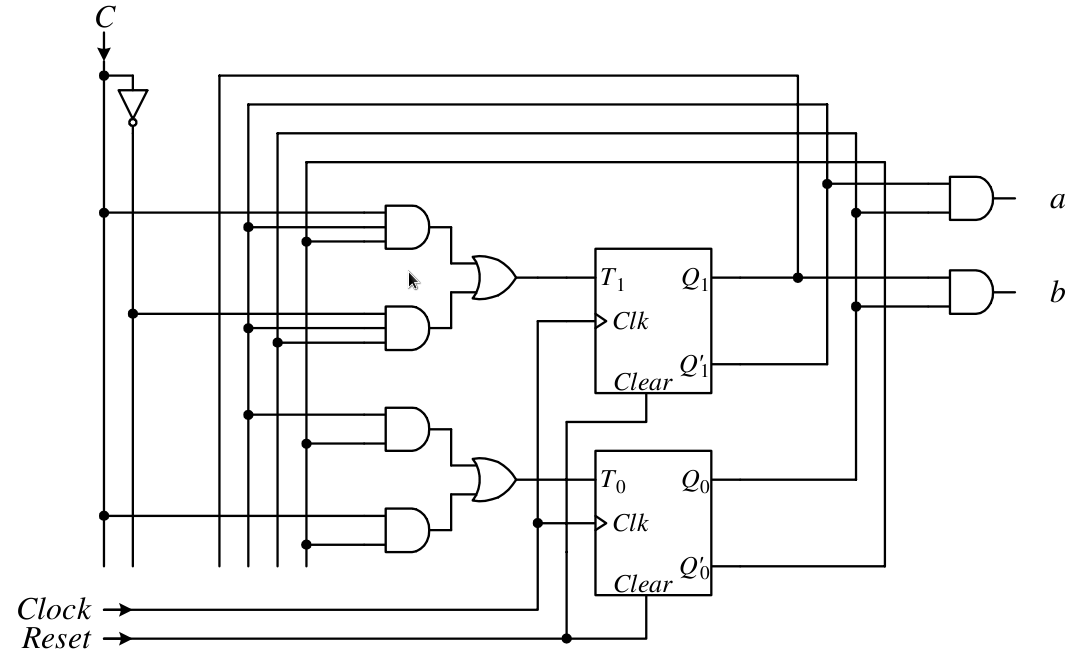
\includegraphics[width = 5in]{p1_q1}
    \end{center}
    
    \item C é uma entrada e a e b são saídas. \\
    \begin{center}
      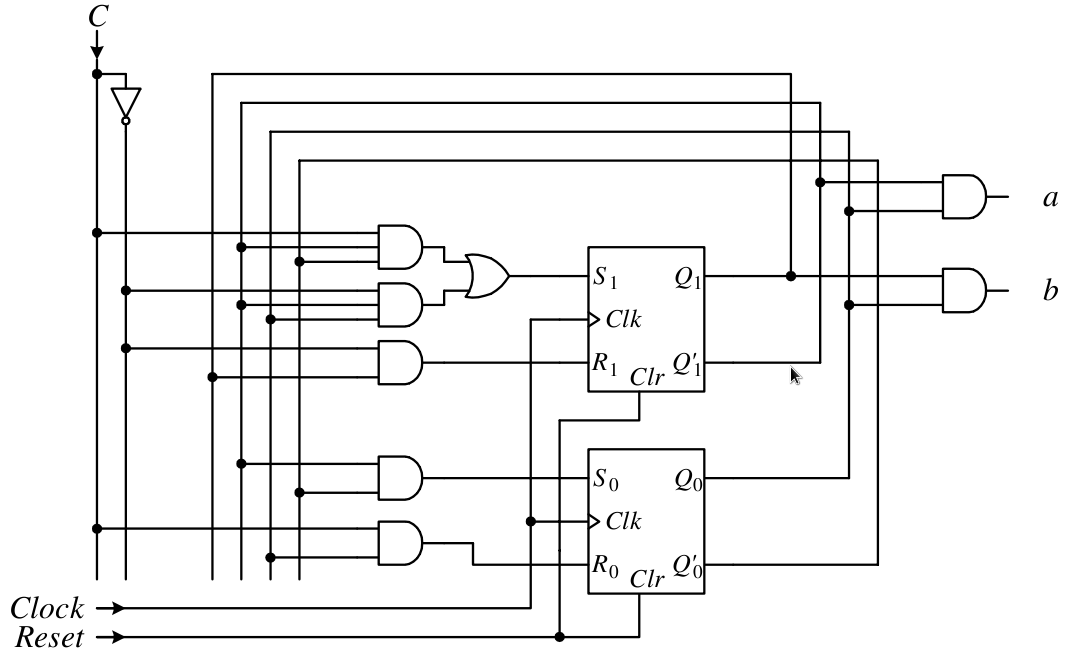
\includegraphics[width = 5in]{p1_q2}
    \end{center}
    
    \item C é uma entrada e a e b são saídas. \\
    \begin{center}
      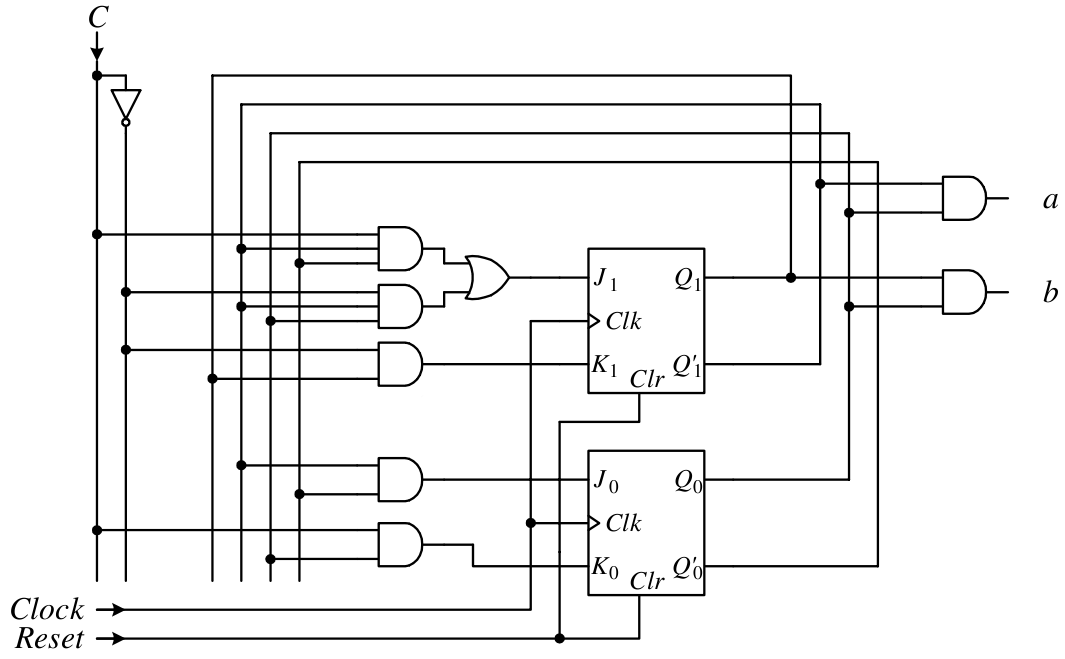
\includegraphics[width = 5in]{p1_q3}
    \end{center}
  \end{enumerate}
  \item Projete um contador módulo 4 utilizando flip-flop T
  \item Projete um contador que conta a seguinte sequência:\\ \textbf{1, 4, 6, 7, 1, 4, 6, 7} \\A contagem deve ser representada diretamente pelo contador de 3 flip-flops. 
	Utilize um flip-flop JK, um flip-flop D e um flip-flop SR, nessa ordem começando pelo bit mais significativo para os 3 flip-flops. O contador é ativado pela 
	entrada C. A contagem para quando C = 0. O próximo estado de todos os estados não utilizados são 
	indefinidos.
  \item Projete um circuito de uma máquina de estado para controlar três interruptores T1, T2, T3 e três lâmpadas L1, L2 e L3. Cada lâmpada é ativada pela opção 
	correspondente, por exemplo, T1 liga a L1. Inicialmente todos os interruptores estão desligados. A primeira opção que é pressionada acende a lâmpada correspondente.
	Quando a primeira lâmpada for ligada, ela permanecerá ligada, enquanto as outras duas lâmpadas permanecem desligadas, e não são afetadas pelas pressões (acionamento) 
	dos contadores subsequenciais até ser reiniciado. 
\end{enumerate}
  
\section{Parte 3}
\begin{enumerate}
 \item Obter o diagrama de estados de um circuito que detecte a paridade de um sinal serial. Considere paridade ímpar e máquina de Moore.
 \item Obter o Diagrama de estados de um circuito de detecte todas sequências 101.\\
  \begin{center}   
    \begin{tabular}{|c|c|c|c|c|c|c|c|c|c|c|c|}
      \hline 
	X & 0 & 1 & 0 & 1 & 0 & 0 & 1 & 0 & 0 & 1 & 0 \\
      \hline
	Z & 0 & 0 & 0 & 1 & 0 & 0 & 0 & 0 & 0 & 0 & 0 \\
      \hline      
    \end{tabular}
  \end{center}
  \item Obter o diagrama de estados de um circuito que indique se o número de 1s recebidos é divisível por 3 (Considerar zero divisível por 3).
      \begin{center}   
    \begin{tabular}{|c|c|c|c|c|c|c|c|c|c|c|c|}
      \hline 
	X & 0 & 1 & 0 & 0 & 1 & 1 & 0 & 1 & 1 & 1 & 0 \\
      \hline
	Z & 1 & 0 & 0 & 0 & 0 & 1 & 1 & 0 & 0 & 1 & 1 \\
      \hline      
    \end{tabular}
  \end{center}
\end{enumerate}

\begin{center}
  \textbf{Bons estudos!!}
\end{center}

\end{document}
